\chapter{System Design}
\section{Precision}
	It's important to have a clear definition of \de{\textit{precision}}, that's different from the concept of \textbf{\textit{accuracy}}: accurate can be seen as a synonymous of a \textit{correctness} (how close we are to the target we want to measure) when instead precise is a synonymous of \textit{consistent} (so when all measures are close together, but not necessarily near to the correct value). In general this two adjectives can be used together in order to create a \textbf{system} that's \textbf{accurate and precise}. In reality it's typically better to design a precise system instead of an accurate one: accuracy can be compensated/calibrated while instead a lack of precision cannot be overcome (and so the precision is an intrinsic property of the system itself).
	
	\begin{figure}[bht]
		\centering 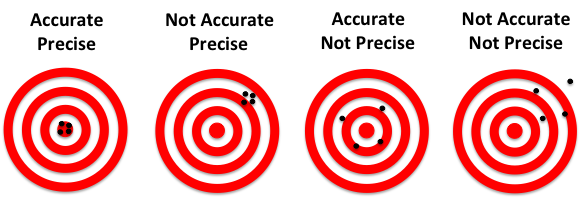
\includegraphics[width=8cm]{acc-prec}
		\caption{accuracy vs precision.}
	\end{figure}
	
	The design of a machine tool or a measurement system has to always consider the \textbf{11 principles for precision} that regards the following key concepts:
	\begin{enumerate}
		\item \textbf{structure}: the structure of the system needs to be stiff with high damping values in order to retain a certain rigidity and thus less degrees of freedom; aspect associated to the structure part are also related to the thermal stability of the system and it's seismic isolation;
		
		\item \textbf{kinematic/semi-kinematic design}: to create a more precisely reliable system  it's necessary to reduce redundant joint between different components (each part has 6 degrees of freedom, but using a joint with more constrains introduce some uncertainty that's the opposite of precision);
		
		\item \textbf{abbé principle}: when aligning measurement system it's important to follow this principle in order not to introduce unexpected side effects;
		
		\item \textbf{direct displacement transducers}: whenever possible it's preferable to measure with a direct transducer, not with a sensor that measure another property that's related to the property itself;
		
		\item \textbf{metrology frames}: this frames that are used to link together the component of the system should be involved in the measurements but should also avoiding the contact with external forces;
		
		\item \textbf{bearings};
		
		\item \textbf{drives/carriages}: in conjunction with the bearings, a system to be put in condition of measure needs to have component with high accuracy that limits the frictions and the thermal effects;
		
		\item \textbf{thermal effects}: whenever possible it's recommended to eliminate/minimise the thermal inputs and drift using stabilization or compensation methods;
		
		\item \textbf{servo drives and control} (CNC): this is a fundamental way to control motion in a repeatable and precise way, especially used in machining systems;
		
		\item \textbf{error budgeting}: in order to improve the way of the system works, it's important to classify different effects in order to understand the relative importance of each effect;
		
		\item \textbf{error compensation}: if it's possible to create a model of the error, it's always good to compensate for it.		
		
	\end{enumerate}
	
	In spite of this 11 principles we realize that, at a fundamental level, there will always be some noise that cannot be eliminated (but can still be reduced). This means that after having designed a system with improved precision it's important to \textbf{identify} and \textbf{quantify} the \textbf{causes leading to non-repeatability}: this is the statistical aspect of precision and represent the so called \textbf{industrial quality}.
	
	\subsection{Autocorrelation}
	
		This day almost all the measures are done using computer and electronic system, so if we consider a displacement sensor it's possible to measure a set of $n$ samples of displacement, each taken after a certain time $\Delta t$. Each sample $x_i$ will necessarily be different from the other, due to it's stochastic nature. At this point to estimate the \textit{real} length of the object to measure we can simply compute the average on the samples token:
		\begin{equation}
			\overline x = \frac 1 n \sum_{i=1} ^n x_i	
		\end{equation}
		This measure will be characterize with a certain variance $\sigma_x^2$; the mean value of the sample will also be a stochastic variable, and so by repeating the experiment itself we can retrieve the variance computed on $m$ measures of $n$ sample each:
		\begin{equation} 
			\sigma^2_{\overline x} = \frac{\sigma_x^2}{m}
		\end{equation}
		
		\begin{SCfigure}[1][bht]
			\centering 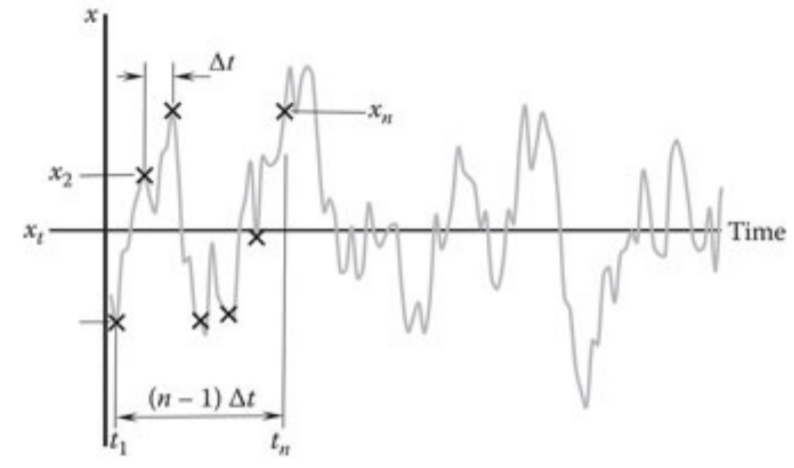
\includegraphics[width=5cm]{autocorrelation}
			\caption{example of values read by a displacement sensor in relation to the time $t$.} \label{fig:design:correlation}
		\end{SCfigure}
	
		As we might see in figure \ref{fig:design:correlation}, reading values in a little time span might result in a correlation between themselves (in fact if we consider a narrow sampling period $\Delta t$, the values registered by the system will be almost be equal), so by increasing the sampling time $\Delta t$ it's possible to get measures that are less correlated between each others. In particular, to solve this problem, it's possible to create the \de{autocorrelation function} $R_{xx}$ whose purpose is to define the minimum sampling time $\Delta t$ that generates uncorrelated data. This particular function is defined by computing the average of a signal with itself translated in time by a constant value $\tau$, so by doing
		\begin{equation}
			R_{xx}(\tau) = \frac 1{T-\tau} \int_0^{T-\tau} x(t) x(t-\tau) \, dt
		\end{equation}
		This particular function is interesting, because we can see that for $\tau = 0$ it simply compute the variance $\sigma_x^2$, however it happens that by incrementing the parameter $\tau > 0$ the function decrease following an exponential decay with time a time constant equal to $\tau_0$ and so the asymptotic value is zero; note that this behaviour is not a true value, but just an asymptotic limit, as it can be seen in figure \ref{fig:design:correlation-b}.
	
		\begin{SCfigure}[1][bht]
			\centering 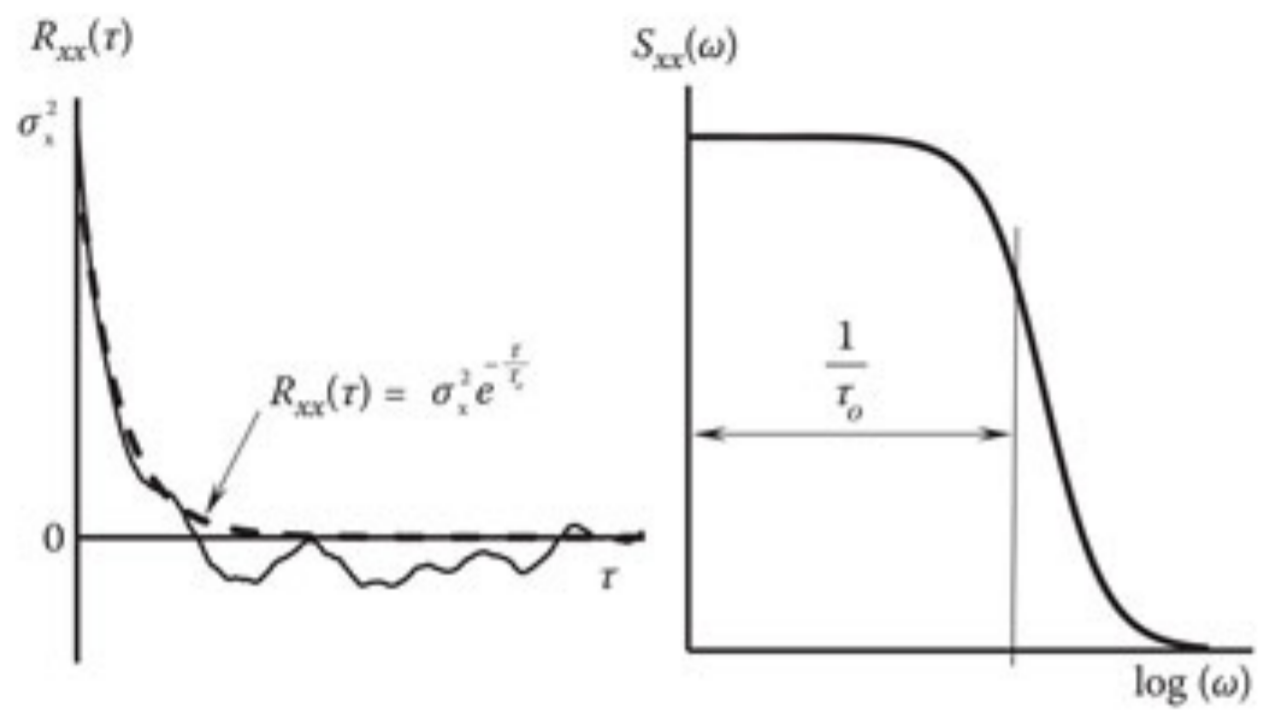
\includegraphics[width=5cm]{autocorrelation-b}
			\caption{trend of the function $R_{xx}$ and $S_{xx}$ read by an instrument.} \label{fig:design:correlation-b}
		\end{SCfigure}
		
		By considering the asymptotic value of the autocorrelation function, so by describing it as $R_{xx}(\tau) = \sigma_x^2 e^{-\frac{|\tau|}{\tau_0}}$ it's possible to compute the power spectral density $S_{xx}$ in the domain of the frequency that's equal to
		\begin{equation}
		\begin{split}
			S_{xx}(\omega) & = \frac{\sigma_x^2}{\pi} \int_0^\infty e^{-\frac{\tau}{\tau_0}} \cos(\omega \tau)\, d\tau = \frac{\sigma_x^2}{\pi \tau_0} \frac 1 {1 + (\omega \tau_0)^2} \\ & = \frac{S_0}{1 + (\omega \tau_0)^2}
		\end{split}
		\end{equation}
		This function is useful to determine that the value $\tau_0$ represents the \textbf{minimum sampling time} for consecutive samples to get the uncorrelated. Going back to the original statement of this section in order to get uncorrelated values we need to use a sampling time $\Delta t > \tau_0$.
		
		By this it consequent that, chosen a time $T$ on which the measure system saves data, the maximum number of uncorrelated sample that can be used for computing some specification on the system is equal to $n = T/\tau_0$, and so with them we can estimate the standard deviation $\sigma^2_{\overline x}$ on the averaged signal:
		\[ \sigma_{\overline x}^2 = \frac{\sigma_x^2}{T/\tau_0} \qquad \Rightarrow \quad \sigma_{\overline x} =\sigma_x \frac{\sqrt{\tau_0}}{\sqrt {T}} = \frac{P_0}{\sqrt {T}} = P_0 \sqrt{(BW)_m} \]
		As stated in this expression, by computing the square root on the variance it's possible to get the standard deviation of the system, and it's possible to see that's related to the \textbf{intrinsic signal noise} $P_0$ (property of the system) and to the square root of the acquisition time $T$ (if on denominator) or on the \textbf{measure bandwidth} $(BW)_m = 1/T$ (if on numerator). \\
		Note that the standard deviation is related to the square root of the acquisition time, so to increase the deviation $\sigma_{\overline x}$ (and so the precision) by a factor of 10, it will require 100 times more time, with a significantly increase of costs.
		
	\subsection{Limits of precision}
		
		As yet described, a limit of precision is the cost because it limit the acquisition time $T$ that could have reduced the standard variation $\sigma_{\overline x}$, but this is not the lonely effect.
		
		Virtually all precision measurements pass through electronics that are subjected to the so called \textbf{Johnson's noise} that's related to the random movement of the atoms that compose the structure, and so in general it depends on the temperature $T$ of the system. Consider for example a resistor $R$, it's thermal noise $P_{0,V}$ depends also on the Boltzamnn's constant $k = 1.38\cdot 10^{-3} J \cdot K^{-1}$ and the sampling bandwidth $(BW)_s$ as described by the equation
		\begin{equation}
			P_{0,V} = 2 \sqrt{RkT (BW)_s}
		\end{equation}
		
		When combining many electric and passive components, their noise sum up to combine into a \textbf{pink noise} (like a white noise, but with more components on higher frequencies) whose spectral density is defined by the function
		\[ G(f) = \frac C f + G_0 \]
		Integrating this function over the frequency band of interest gives the variance $\sigma^2_V$ associated to this particular kind of noise
		\begin{equation}
			\sigma_V^2 = \int_{f_1}^ {f_2} G(f)\, df = C \ln \left( \frac{f_1}{f_2} \right) + G_0 \big(f_2-f_1\big)
		\end{equation}
		The truth that this equation wants to tell us it that is difficult to maintain precision over a long time, because the difference of frequencies $f_2-f_1$ (multiplied by $G_0$) will increase the variance.
		
		Another phenomenon that limit the precision of an instrument is the granular nature of current (that's made of flowing electrons); this effect is dominant for high currents $I$ and bandwidth $(BW)_s$ and determine a so called \textbf{shot noise} $P_{0,I}$ that's equal to		
		\[ P_{0,I} = \sqrt{2qI (BW)_s}\]
		where $q = 1.602\cdot 10^{-19} C$ is the charge of an electron.		
		\vspace{3mm}
		
		Pink noise and shot noise are the limiting factors on precision measurements where a phenomenon is converted through a transducer into a voltage or current. Much better precision can be exploited by converting a phenomenon into a value through time (needed, as example, for charging a capacitor or for a beam of light to travel a distance...) and not voltage/current; this time precision can reach value of $10^{-11} s$, increasing the precision of the overall system.
	
	
	
	
	
	
	
	
	
	
	
	
	
	
	
	
	
	
